\section{Checkning av checklistor - Robin Andersson}
\subsection{Inledning}
Vårt system ska innehålla två olika typer av checklistor på olika webbsidor. Om flera användare är inne på samma sida samtidigt och en person checkar en checkruta så ska den checkrutan bli checkad för alla användare som är inne på den webbsidan.

Den ena typen av checklista är en plocklista där det finns information om vilka engångsmatrial som behövs för den operationsförberedelse som användaren är inne på samt vart de matrialen kan hämtas någonstans. När en sjuksköterska har plockat en artikel så checkar denne av den artikeln i plocklistan.

Den andra typen av checklista är en lista av operationssalsförberedelser där det kan stå en längre beskrivning om vad som ska göras och när en sjuksköterska har utfört hela den förberedelsen så checkar denne av den förberedelsen i förberedelselistan.

Checklistorna kommer att implementeras med hjälp av handlebars, javascript, jquery samt Socket.IO. För information om dessa språk/paket hänvisar jag till bakgrunden i den gemensamma rapporten.

\subsubsection{Syfte}
Syftet med denna del av projektet är att flera sjuksköterskor samtidigt ska kunna förbereda operationer genom att plocka olika artiklar samt förbereda operationssalen och checka av det som är utfört utan att det ska bli några konflikter med att flera sjuksköterskor plockar samma artikel eller liknande.

\subsubsection{Frågeställning}
\begin{itemize}
\item Går det att anpassa checklistan för en surfplatta medan den samtidigt innehåller information om var artiklar befinner sig samt hur många av varje artikel som behövs?

\item Kommer Socket.IO vara tillräckligt snabbt för att flera personer ska kunna checka av artiklar samtidigt utan förvirring?
\end{itemize}

\subsubsection{Avgränsningar}
Eftersom denna del av projektet endast innehåller checkande av checklistor så saknas etiska aspekter.

\pagebreak
\subsection{Teori}
\subsubsection{Websockets}
WebSockets består av ett nätverksprotokoll och ett API som gör det möjligt att skapa en WebSocket uppkoppling mellan en klient och en server. Med hjälp av WebSocket API:t så kan man hantera en full-duplex kanal som kan användas till att skicka och ta emot meddelanden. En WebSocket anslutning skapas genom att gå över från HTTP protokollet till WebSockets nätverksprotokoll när en initial handskakning mellan server och klient sker. När en WebSocket anslutning finns uppkopplad så kan WebSocket meddelanden skickas fram och tillbaka mellan metoderna som finns definierade i WebSockets gränssnitt. När WebSockets används i ett system så används asynkrona eventlyssnare för att lyssna på kommunikationen. WebSockets API är rent eventbaserat villket betyder att klienter inte behöver kontrollera om servern har uppdaterats utan att de istället uppdaterar när de får ett event. \cite{websocketbook}

Kanalen som WebSocket använder sig av kommunicerar över nätet med hjälp av en enda socket. WebSockets använder sig av väldigt mycket mindre trafik och har mycket kortare latens än Ajax. WebSockets använder sig av de vanliga HTTP portarna (det vill säga port 80 och port 443) \cite{websocketreport}

Huvuddelen av denna del av projektet handlar om kommunikation med Socket.IO som använder sig utav WebSockets för att kommunicera mellan server och klienter.

\pagebreak
 
\subsection{Metod}
Jag började med att fundera på hur kommunikationen skulle fungera på för sätt. Jag skissade ner olika förslag på ett papper och kom på det sättet fram till hur jag skulle implementera kommunikationen. Sedan implementerade jag den och fick den att fungera för plocklistan. Därefter så refaktoriserade jag koden för att få den kortare och mer lättläst. När plocklistan sedan var färdig implementerad så började jag fundera på hur jag skulle kunna använda mig av så mycket kod som möjligt från plocklistan till att implementera förberedelselistan. Efter det att jag implementerat förberedelselistan så refaktoriserade jag igen för att få koden mer lättläst.

\subsection{Resultat}
Jag kom fram till att när en användare går in på en operationsförberedelse så kommer denne in i ett rum. Varje gång en person sedan checkar en checkbox så skickas ett Socket.IO meddelande till servern som innehåller information om vilken checkruta som ska checkas samt vilket rum checkboxen ska checkas i. Servern skickar sedan ett meddelande till det givna rummet vilken checkruta som ska checkas och alla klienter som är anslutna till det rummet checkar den givna checkrutan.

Figuren nedan visar detta flöde i ett sekvens liknande box-and-line-diagram.
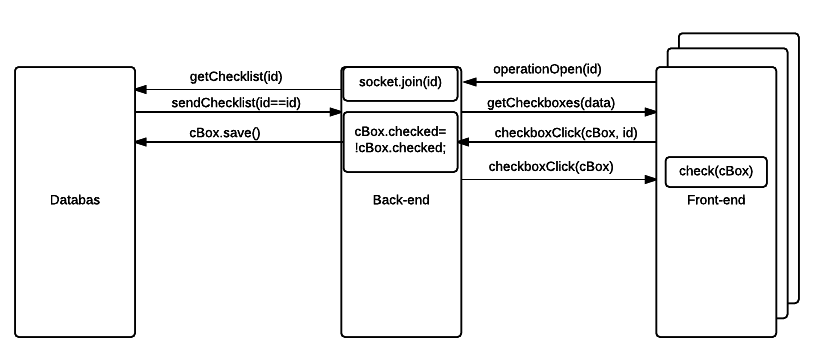
\includegraphics[scale=0.5]{checklistdiagram}

När två klienter går in på en operation och en klient checkar en checkruta för första gången tar det strax under en sekund innan checkrutan checkas för den andra klienten. Därefter när någon klient checkar en checkruta så kan jag inte se någon fördröjning alls från det att en klient checkar en checkruta och en annan klient får den checkrutan checkad.

Kunden har prövat att ha flera personer inne på samma plocklista samtidigt och checka av olika artiklar. Kunden tyckte att det fungerade bra och påpekade inte någon fördröjning. 

All information som krävs för plocklistorna fick plats med mycket mellanrum och upplevs därav inte som plottrigt.

\subsection{Diskussion}
\subsubsection{Resultat}
Eftersom jag endast skickar data om vilken checkruta som ska checkas till de klienter som är inne på den operation som checkrutan blev checkad på så uppdateras checkningar snabbare än att göra den enkla lösningen att bara skicka datat till alla anslutna klienter. Att det tar nästan en sekund för en checkning att uppdateras på andra klienter för första gången är långsammare än förväntat. Men eftersom det endast gäller just första artikeln och att kunden har testat checkning med flera personer samtidig utan att märka några problem så verkar detta inte vara något praktiskt problem. Att en checkning sedan kan uppdateras nästan helt utan fördrdröjning var bättre än vad jag hade förväntat mig.

\subsubsection{Metod}
Den metod jag använde mig av fungerade bra, men jag tror att jag skulle kunnat komma fram till samma resultat snabbare genom att göra kortare funktioner och vettigare namn redan från början istället för att göra något som funkar så snabbt som möjligt och sedan refaktorisera. För nu blev det väldigt förvirrande kod från början och jag var tvungen att sitta och tänka på vad kod jag skrivit faktiskt gjorde. Men att skissa olika förslag på ett papper först tror jag var en väldigt bra idé, det gjorde att jag fick några möjliga lösningar och sedan kunde jag överväga fördelar och nackdelar med de olika lösningarna för att sedan välja den som verkade bäst.

Att jag började med att implementera plocklistan och inte förän den var klar implementera förberedelselistan tror jag också var en bra idé. Jag kunde då till en början fokusera på en typ av checklista och se till att få den att fungera bra. Sedan när förberedelselistan skulle implementeras så kunde jag återanvända väldigt mycket av den kod som jag skrivit till plocklistan.
\pagebreak
\subsection{Slutsatser}
All nödvändig information i plocklistorna fick plats med bra marginal, därav anser jag att svaret på min första frågeställning är: Ja!

Jag har lyckats implementera checkning av både plocklistor och förberedelselistor med ungefär samma kod. Checkningen uppdateras för alla klienter som är inne i samma operationsförberedelse. Det är nästan en sekunds fördröjning när en person checkar den första checkrutan i en checklista tills dess att de andra anslutna klienterna får den checkrutan checkad. Efter det att den första rutan är checkad så uppdateras checkningar utan märkbar fördröjning till de andra anslutna klienterna. Därav anser jag att svaret på min andra frågeställning är: Ja!

Eftersom kunden har prövat checkningen av cheklistor med flera personer samtidigt och de tyckte att den fungerade bra som helhet så anser jag att syftet med denna del av projektet är upplevt.

%\subsection{Referenser}
%\vspace{-9mm}
%\begin{thebibliography}{9}
%\bibitem{websocketbook} Wang Vanessa, Salim Frank, Moskovits Peter; The Definitive Guide to HTML5 WebSocket; New York City APress, 2013.
%\bibitem{websocketreport} http://www.scirp.org/journal/PaperInformation.aspx?PaperID=25428
%\end{thebibliography}